\section{DDoS Dissector}
\label{sec:ddos_dissector}
%about fingerprint: concepts \& context}

There are several words used in academia and the security community for what we will define as a DDoS attack fingerprint. The words are DDoS `characteristics', `fingerprint', `profile', `pattern', `signature', and `rule'. Oxford dictionary defines these words as the following:

\begin{itemize}
	\item \textbf{characteristics}: ``a feature or quality belonging typically to a person, place, or thing and serving to identify them'';
	\item \textbf{profile}: ``a graphical or other representation of information relating to particular characteristics of something, recorded in quantified form'';
	\item \textbf{pattern}: ``a regular and intelligible form or sequence discernible in the way in which something happens or is done'';
	\item \textbf{signature}: ``a distinctive pattern, product, or characteristic by which someone or something can be identified'';
	\item \textbf{rule}: ``a principle that operates within a particular sphere of knowledge, describing or prescribing what is possible or allowable'';
\end{itemize}

We will however use an umbrella term, a \textbf{fingerprint}, from which the above five can be derived. A fingerprint is the smallest set of features that summarizes the main characteristics of each attack vector in a DDoS attack, extracted from a network measurement of the attack.

The goal of determining the fingerprint is to extract a distinct set of properties that allow us to identify the attack (see figure \ref{fingerprint}). This set can later be used as a signature for a signature-based firewall, or to identify the source of the attack. We distinguish two types of properties, namely \emph{a priori} and \emph{a posteriori} properties. We assume that all packets are IP-based packets, so no AppleTalk or other legacy protocols. With that assumption, the following a priori properties are known for each packet: (1) type (TCP/UDP); (2) protocol (DNS, HTTP, etc.); (3) extra attributes based on the protocol; (4) source port; (5) destination port; (6) source IP; (7) destination IP. Once we have established the type of attack, for example UDP/DNS from port 23 from IP addresses \textit{x}, \textit{y} and \textit{z}, we can determine several higher level properties, namely (1) the amount of packets per second; (2) the start time; (3) the duration. The low and high level properties together will be defined as a priori properties. With just the a priori properties, we can determine several a posteriori properties, such as the origin country of the IP addresses, autonomous system, whether the IP addresses are known for other malicious behaviour and whether the IP addresses were spoofed. The a priori and a posteriori information combined creates an attack vector. A DDoS attack is composed of one or more single vector attacks. All single vectors of a DDoS attack are linked to one multivector key.

\begin{figure}
\begin{lstlisting}
{
  protocol: "DNS",
  additional: {
    dns_query: "example.org",
    dns_type: 255
  },
  src_ips: [
    {
      as: "1234"
      ip: "100.64.52.11"
      cc: "XX"
    }
    ...
  ],
  total_src_ips: 34,
  src_ports: [
    53
  ],
  total_src_ports: 1,
  dst_ports: [
    24018,
    5441
    ...
  ],
  total_dst_ports: 17132,
  key: "1a79a4d60de6718e8e5b326e338ae533",
  start_time: "2019-02-30 12:00:00",
  duration_sec: 35.794759473957483,
  avg_pps: 627.9138370201783,
  avg_bps: 1535724.0964006053,
  vector_filter: "...",
  multivector_key: "66b375b08fc869336..."
} 
\end{lstlisting}

\caption{An example of an enriched fingerprint for one attack vector. The enriched part is the extra information about the IP, i.e. the Autonomous System number (AS) and country code (CC)}
\label{fingerprint}
\end{figure}

Now that we have defined what an attack vector consists of, we will outline the way to retrieve aforementioned properties from a packet capture. 
\begin{enumerate}
	\item The first step is determining the destination IP of the attack. Generally, this will be the most frequent destination IP address.
	\item Next, we determine the most frequent protocol used for the attack, e.g. DNS. 
	\item Lastly, the source and destination ports are determined. The relation of source and destination ports is generally one-to-many, one-to-one, or many-to-one. In rare cases, the ports have a many-to-many relationship.
\end{enumerate}
Based on these parameters, the packets belonging to the attack are extracted, the results are removed from the set and the process runs again, until there is no further probable attack vector left. This set of attack vectors gives us a key insight in the fingerprinting process. For instance, it can tell us the starting time of the attack, the amount of packets per second and more. 

However, we still need to anonymize the data. After all, the victim would rather remain unknown, as the attack information is often sensitive. We do this by overwriting all destination IP data from the extracted data by 0 bytes. The destination IP can be safely removed as it is not part of the fingerprint, and provides no other value to our analysis.

We wish to minimize the amount of processing required during an attack, so all a priori properties are determined while the attack is happening, whilst the a posteriori properties are gathered after the attack has passed. This process can be done after the anonymised attack vector is uploaded to DDoSDB.

\begin{figure}
	\centering
	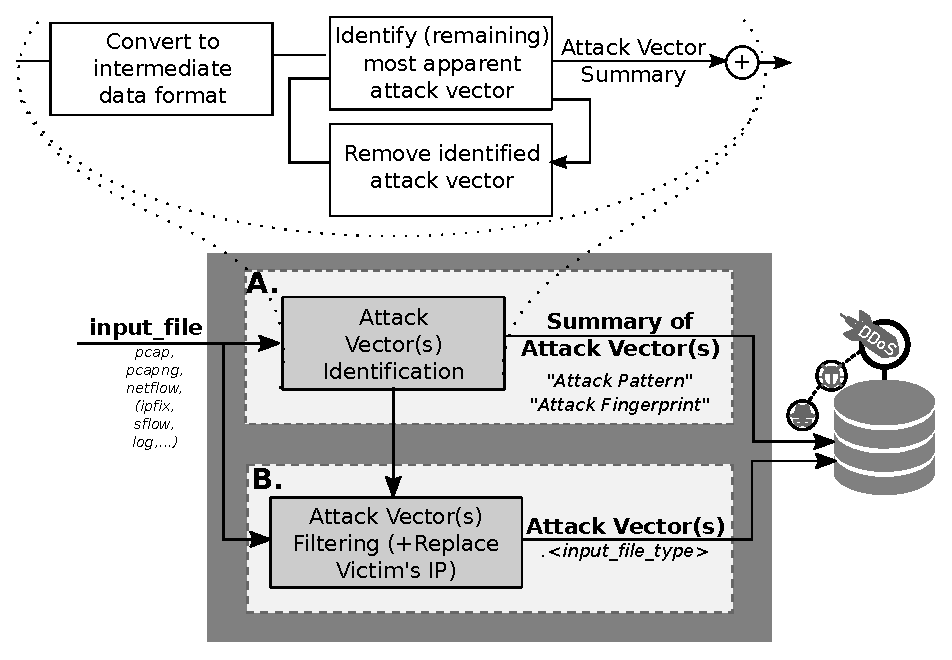
\includegraphics[width=0.5\textwidth]{{figs/ddos_fingerprinting.eps}}
	\caption{Process overview of the DDoS Dissector attack vector extraction}
\end{figure}







 
